\documentclass{article}
\usepackage[a4paper, margin=3mm, landscape]{geometry}
\usepackage{multicol}
\usepackage{xcolor}
\usepackage{enumitem}
\usepackage{amsmath}
\usepackage{amsfonts}
\usepackage{listings}
\usepackage{soul}
\usepackage{graphicx}

\pdfinfo{
    /Title (CS4243.pdf)
    /Creator (TeX)
    /Producer (pdfTeX 1.40.0)
    /Author (Jason Qiu)
    /Subject (CS4243)
    /Keywords (CS4243, nus, cheatsheet, pdf)
}

\graphicspath{ {./img/} }

\pagestyle{empty}
\setcounter{secnumdepth}{0}
\setlength{\columnseprule}{0.25pt}

% Redefine section commands to use less space
\makeatletter
\renewcommand{\section}{\@startsection{section}{1}{0mm}%
    {-1ex plus -.5ex minus -.2ex}%
    {0.5ex plus .2ex}%x
{\normalfont\large\bfseries}}
\renewcommand{\subsection}{\@startsection{subsection}{2}{0mm}%
    {-1explus -.5ex minus -.2ex}%
    {0.5ex plus .2ex}%
{\normalfont\normalsize\bfseries}}
\renewcommand{\subsubsection}{\@startsection{subsubsection}{3}{0mm}%
    {-1ex plus -.5ex minus -.2ex}%
    {1ex plus .2ex}%
{\normalfont\small\bfseries}}%
\makeatother

% Adjust spacing for all itemize/enumerate
\setlength{\leftmargini}{0.5cm}
\setlength{\leftmarginii}{0.5cm}
\setlist[itemize,1]{leftmargin=2mm,labelindent=1mm,labelsep=1mm}
\setlist[itemize,2]{leftmargin=2mm,labelindent=1mm,labelsep=1mm,label=$\bullet$}
\setlist[itemize,3]{leftmargin=2mm,labelindent=1mm,labelsep=1mm,label=$\bullet$}

% Font
\renewcommand{\familydefault}{\sfdefault}

% Define colors for math formulas
\definecolor{myblue}{cmyk}{1,.72,0,.38}
\everymath\expandafter{\the\everymath \color{myblue}}

% Custom command for keywords
\definecolor{highlight}{RGB}{251,243,218}
\newcommand{\keyword}[2]{\sethlcolor{highlight}\hl{\textbf{#1}} - #2}
\newcommand{\ilkeyword}[1]{\sethlcolor{highlight}\hl{\textbf{#1}}}

% Define colors and style for code
\definecolor{codegreen}{rgb}{0,0.6,0}
\definecolor{codegray}{rgb}{0.5,0.5,0.5}
\definecolor{codered}{HTML}{CC241D}
\definecolor{backcolor}{rgb}{0.95,0.95,0.95}
\lstdefinestyle{codestyle}{
    backgroundcolor = \color{backcolor},
    commentstyle = \color{codegray},
    keywordstyle = \color{codered},
    stringstyle = \color{codegreen},
    basicstyle = \ttfamily,
    breakatwhitespace = false,
    showstringspaces = false,
    breaklines = true,
    showtabs = false,
    tabsize = 2
}
\lstset{style = codestyle}

% -----------------------------------------------------------------------
\begin{document}
\begin{multicols*}{4}
\footnotesize

% Title box
\begin{center}
    \fbox{
        \parbox{0.8\linewidth}{
            \centering \textcolor{black}{
                {\Large\textbf{CS4243}} \\
                \normalsize{AY23/24 Sem 2}} \\
                {\footnotesize \textcolor{gray}{github.com/jasonqiu212}}
        }
    }
\end{center}

\section{05. Segmentation}

\begin{itemize}
    \item Goal: Separate image into coherent regions
    \item Idea: \keyword{Clustering}{Group similar data points together}
    \item Challenges: What makes 2 points same/different? Choice of features (e.g. Color, Intensity, Position), Which clustering algorithm?
    \item \keyword{k-Means Clustering}{Iteratively re-assign points to nearest cluster center}
    \begin{enumerate}
        \item Given $K$, randomly initialize the cluster centers $c_1, \ldots, c_K$
        \item For each point $p_i$, find the closest $c_j$ and put $p_i$ into cluster $j$
        \item Set $c_j$ to be mean of points in cluster $j$
        \item Repeat, if $c_j$ have changed up to some threshold
    \end{enumerate}
    \begin{itemize}
        \item Pros: Simple, Converges to local min.
        \item Cons: Setting $K$, Sensitive to initial centers (Since k-means converges to local min.), Sensitive to outliers (Can add more clusters), Assumes spherical clusters (Fix with mean-shift)
    \end{itemize}
    \item \ilkeyword{Simple Linear Iterative Clustering (SLIC) Superpixels}
    \begin{itemize}
        \item \keyword{Superpixel}{Group of pixels that share common traits}
        \begin{itemize}
            \item Application: Inputs to other CV algo. since more compact representation with perceptual meaning
        \end{itemize}
        \item Num. of pixels: $n_{tp}$; Target num. of superpixels: $n_{sp}$
        \item Initial width of each superpixel: $s = \sqrt{\frac{n_{tp}}{n_{sp}}}$
        \item Features: $z = [r,g,b,x,y]$
        \item Color distance: $d_c = || \langle r_j,g_j,b_j \rangle - \langle r_i,g_i,b_i \rangle ||$
        \item Spatial distance: $d_s = || \langle x_j,y_j \rangle - \langle x_i,y_i \rangle ||$
        \item Scaling factors: $d_{cm}$ and $d_{sm}=s$ set as max. expected values of $d_c$ and $d_s$ respectively
        \item $D = \sqrt{(\frac{d_c}{d_{cm}})^2+(\frac{d_s}{d_{sm}})^2} = \sqrt{d_c^2 + (\frac{d_s}{s})^2 c^2}$
    \end{itemize}
    \begin{enumerate}
        \item Split img. into grid of size $s \times s$. Set cluster centers as lowest gradient position in $3 \times 3$ neighborhood from superpixel center to speed up convergence since initialize on value common to surrounding.
        \item For each cluster center, check distance to all pixels within $2s \times 2s$ neighborhood. Assign pixels to closest checked center.
        \item Update cluster centers using mean and repeat if not converged (Same as k-Means)
        \item Optional: Replace superpixel region by average value to create stained glass effect
    \end{enumerate}
    \begin{itemize}
        \item Modification of k-Means: Not random initialization, Compute pixel's distance only to closest set of cluster centers
        \item Can enforce connectivity and use other features too
    \end{itemize}
    \item \keyword{Mean-Shift Clustering}{Find local density maxima in feature space}
    \begin{itemize}
        \item \keyword{Attraction basin}{Region in feature space for which all trajectories of centroids lead to same mode}
        \item \keyword{Cluster}{All data points in attraction basin of a mode}
    \end{itemize}
    \begin{enumerate}
        \item For each data point:
        \begin{enumerate}
            \item Define window around and get centroid
            \item Shift window to centroid
            \item Repeat until window centroid stops moving
        \end{enumerate}
    \end{enumerate}
    \begin{itemize}
        \item Segmentation with Mean Shift: Do mean shift and merge pixels in same attraction basin
        \item Choosing window size: Trial and error, Sample points and use avg. dist. to knn. (Num. of neighbors needs to be large enough to ensure increase in density)
        \begin{itemize}
            \item Larger window size $\rightarrow$ Fewer clusters
        \end{itemize}
        \item Pros: No assumptions on cluster shape, 1 parameter, Finds variable num. of modes (vs. specified $k$ in k-Means), Robust to outliers
        \item Cons: Choosing $h$, Slow, Scales poorly with feature space dimension
        \item Optimizations:
        \begin{itemize}
            \item After each run of mean shift, assign all points within radius $r$ of end point to same cluster
            \item Assign all points within radius $c < r$ of search path to mode $\rightarrow$ More aggressive, less confident
        \end{itemize}
    \end{itemize}
\end{itemize}

\section{06. Texture}

\begin{itemize}
    \item \keyword{Texture}{Pattern with repeating elements}
    \item \keyword{Filter Bank}{Measures variety of structures in local neighborhood and generates multi-dimensional features}
    \begin{itemize}
        \item Goal: How to represent texture?
        \item Idea: Apply filters with small windows to generate statistics that summarize local patterns. Dist. in feature space bet. windows $\rightarrow$ Pixel's texture similarity
        \item $d$ filters $\rightarrow$ $d$-dimensional feature vector
        \item Choosing window size: Try many sizes and look for one where statistic does not change much
        \item Choose filters in different scales and orientations (to solve window size problem)
        \item \keyword{Gabor Filter}{Represent filter banks mathematically by combining sinusoids with exp. (Gaussian) envelope}
    \end{itemize}
    \item \keyword{Texton}{Characterizes texture by replacing each pixel with integer representing \textbf{texture type}}
    \begin{enumerate}
        \item Apply filter bank to training image
        \item Cluster in feature space and store cluster centers (Texton dictionary)
        \item For test image, filter image with same filter bank to get feature vector for each pixel. Assign each pixel to nearest cluster. Cluster ID = Texton ID.
        \item For a given region, compute \ilkeyword{texton histograms}
    \end{enumerate}
    \begin{itemize}
        \item Classification: Given new img., compare hist. to other trng. samples and assign to label with most similarity
        \item Segmentation: Use texton histograms as a feature
    \end{itemize}
    \item \keyword{Perceived Boundaries}{Segmentation by human}
    \begin{itemize}
        \item Idea: Texture gradients indicate boundaries well
    \end{itemize}
    \begin{enumerate}
        \item For each pixel, consider a disk that is split into 2 halves with some orientation
        \item Measure texture diff. bet. 2 halves via texton hist.
        \item Try all orientations. Orientation with high difference suggests boundaries.
    \end{enumerate}
\end{itemize}

\section{07. Keypoints}

\begin{itemize}
    \item Motivation: How to stitch 2 images (e.g. Panaroma)?
    \begin{enumerate}
        \item Keypoints: Find locations
        \item Descriptors: Rep. surrounding regions with math
        \item Homography: Do the matching
    \end{enumerate}
    \item Good keypoints are \textbf{repeatable} and \textbf{distinct}
    \item \ilkeyword{Harris Corner Detection}
    \begin{itemize}
        \item Significance: Corners have big changes in all directions when shifting window
        \item Given window $W$ shifted by offset $(u,v)$:
        \[
            E(U,v)=\sum_{(x,y) \in W} (I(x+u,y+v) - I(x,y))^2
        \]
        \item Assuming only small shifts (for Taylor Series Exp.):
        \[
            E(u,v) = Au^2 + 2Buv + Cv^2 = \begin{vmatrix}
                u & v \\
            \end{vmatrix}
            \begin{vmatrix}
                A & B \\
                B & C \\
            \end{vmatrix}
            \begin{vmatrix}
                u \\
                v \\
            \end{vmatrix}
        \]
        \begin{itemize}
            \item $A = \sum_{(x,y) \in W} I_x^2$ $\quad$ $B = \sum_{(x,y) \in W} I_x I_y$
            \item $C = \sum_{(x,y) \in W} I_y^2$
            \item \keyword{2nd Moment Matrix (H)}{Middle matrix}
        \end{itemize}
        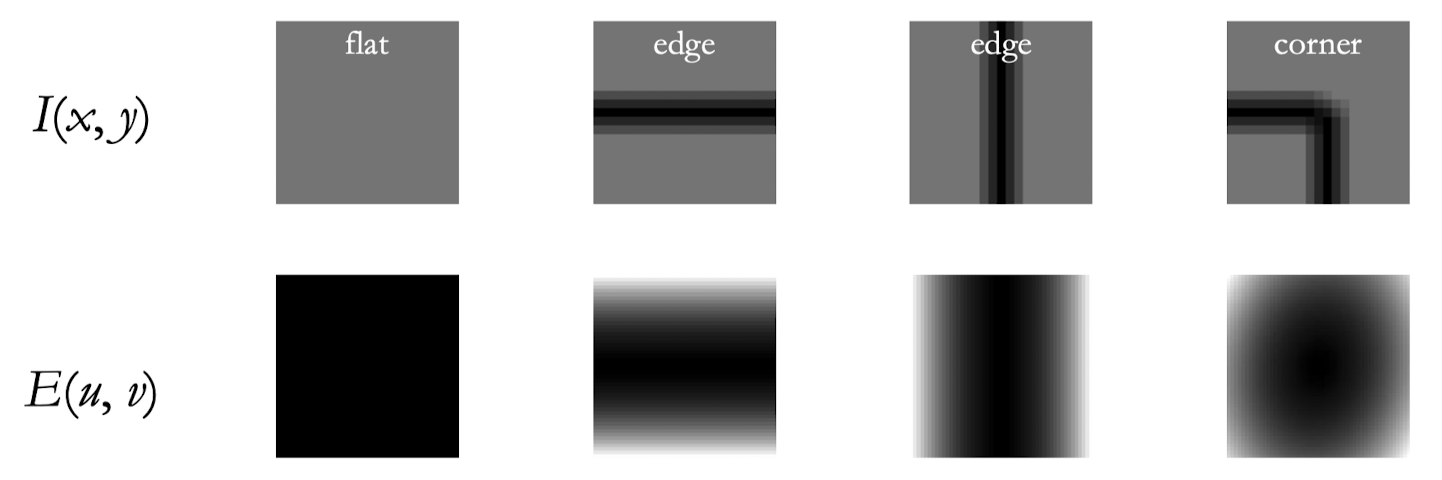
\includegraphics[scale=0.22]{corner-ssd-error.jpg}
        \item $E = k$ visualized as ellipse, where $H$ controls shape
            \begin{itemize}
                \item Eigenvectors of $H$ $\rightarrow$ Axes orientation
                \item Eigenvalues of $H$ $\rightarrow$ Axes length
            \end{itemize}
        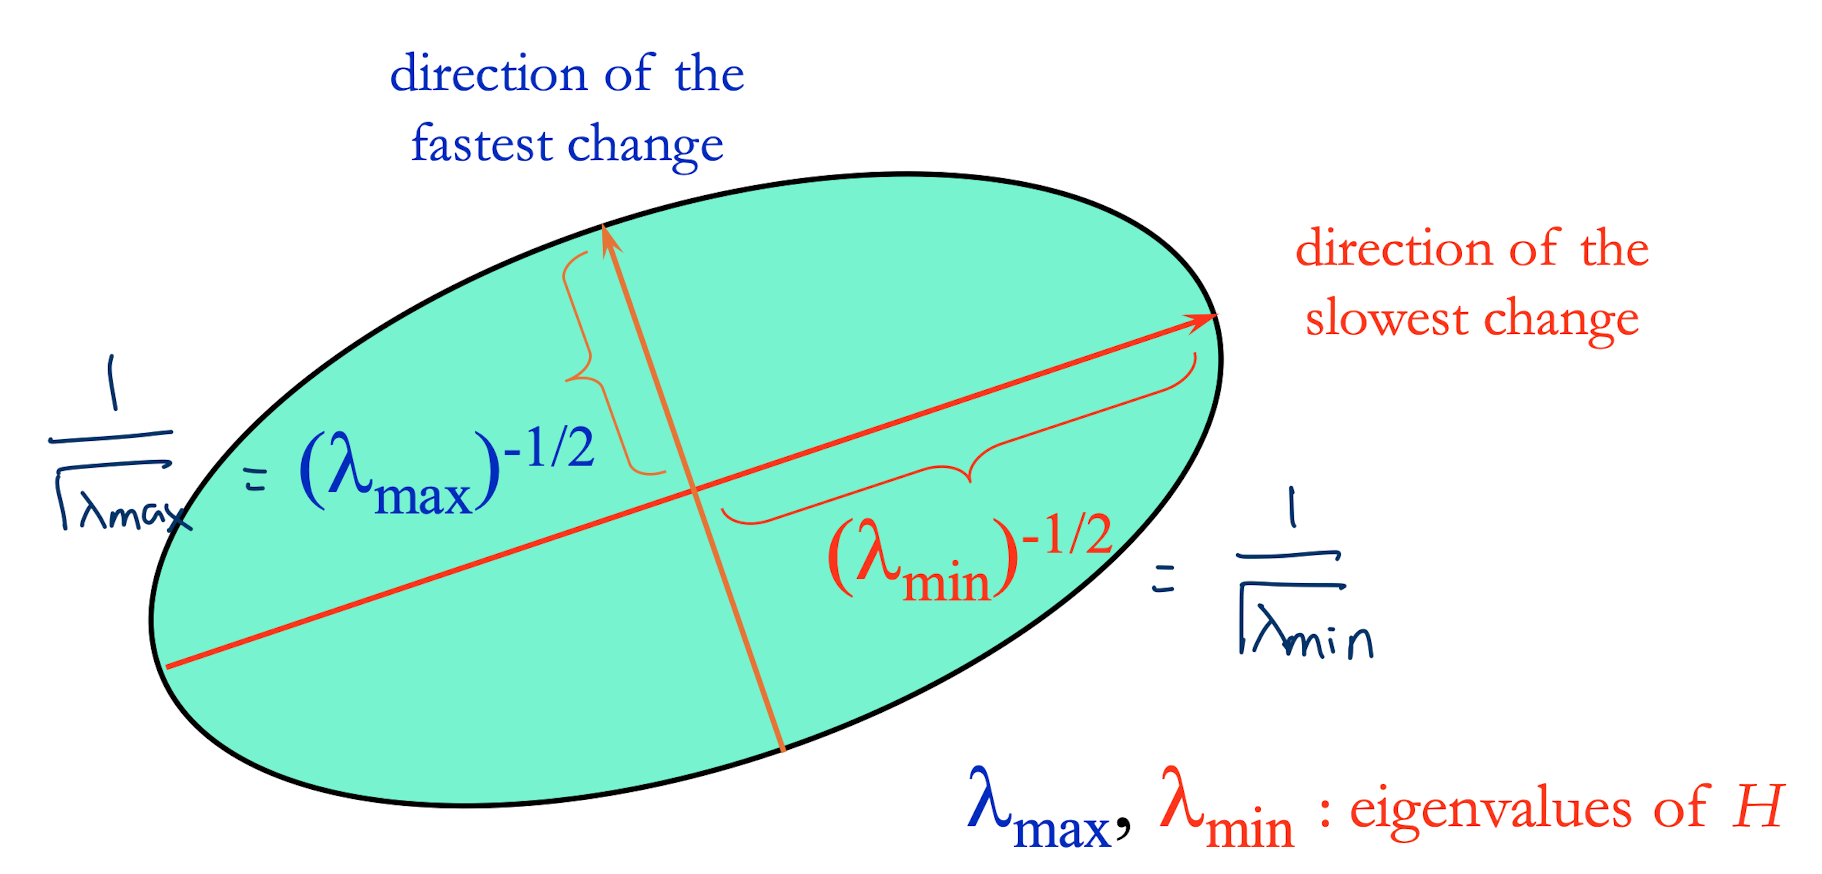
\includegraphics[scale=0.18]{h-ellipse.jpg}
        \item \ilkeyword{Eigenvectors} of $A$ are vectors $\mathbf{x}$ that: $A\mathbf{x} = \lambda \mathbf{x}$
        \item \ilkeyword{Eigenvalue ($\lambda$)} corresponds to $\mathbf{x}$: $\det(A-\lambda I) = 0$
        \item Since $A = H$ is $2 \times 2$: $\lambda_{\pm} = \frac{1}{2} ((h_{11} + h_{22}) \pm \sqrt{2h_{12}h_{21} + (h_{11} - h_{22})^2})$
        \item After getting $\lambda$s, find $\mathbf{x}$: $(A - \lambda I) \mathbf{x} = 0$
        \item Both $\lambda_{\text{max}}$ and $\lambda_{\text{min}}$ are large $\rightarrow$ Corner
        \item 'Cornerness' Score: $R = \min(\lambda_1, \lambda_2)$ (But getting $\lambda$ is slow)
        \item \ilkeyword{Harris Operator}: $R = \det (H) - \kappa (\text{trace}(H))^2$
        \begin{itemize}
            \item $\det (H) = AC - B^2 = \lambda_1 \lambda_2 $
            \item $\text{trace} (H) = A + C = \lambda_1 + \lambda_2 $
            \item $R > 0$ $\rightarrow$ Corner, $R<0$ $\rightarrow$ Edge, $R \approx 0$ $\rightarrow$ Flat
        \end{itemize}
        \begin{enumerate}
            \item Compute gradient for each point in image
            \item Compute $H$ matrix for each image window and get 'correctness' score
            \item Find points with window where $R > $ threshold
            \item Take points of local maxima
        \end{enumerate}
        \item \keyword{Non-Max. Suppression}{Iteratively search for max. values, then zero everything in surrounding window}
        \begin{itemize}
            \item Window size important
            \item Adaptive: To prevent uneven distri. of keypoints in areas of higher contrast, pick corners which are both local max. and whose response is greater than all neighboring local max.
        \end{itemize}
        \item In practice, $H = \sum_{(x,y) \in W} w_{x,y} \begin{vmatrix}
            A & B \\
            B & C \\
            \end{vmatrix}$ (Gaussian)
    \end{itemize}
    \item \ilkeyword{Harris Corner Invariances}
    \begin{itemize}
        \item Purpose: If img. transf., how repeatable is detection?
        \item \keyword{Equivariance}{Image transformed, and detection location undergoes similar transformation}
        \item \keyword{Invariance}{Image tranf., but no detection score change}
        \item Translation: Equivariant and invariant
        \item Rotation: Equivariant and invariant
        \item Photometric transformation (Assume $I' = aI + b$): Invariant to $b \neq 0$, but not invariant to $a \neq 1$
        \item Scaling: Not equivariant (i.e. Img. scaled up)
        \begin{itemize}
            \item Scale of window can determine if location is keypoint $\rightarrow$ Need to scale up window by image scale
            \item \keyword{Auto. Scale Selection}{When looking for keypoints, try window sizes and find scale that gives local max.}
        \end{itemize}
    \end{itemize}
    \item \keyword{Laplacian of Gaussian}{Alternative keypoint detector which detects 'blobs' and is scale-sensitive}
    \begin{itemize}
        \item $\nabla^2 g = \frac{\partial^2 g}{\partial x^2} + \frac{\partial^2 g}{\partial y^2}$
        \item Idea: Convolution with LoG has highest response when signal has same scale as Gaussian. Built-in scale sensitivity by varying scale $\sigma$.
        \item Implementation: Fix window and kernel size; rescale img. with Gaussian blurring and downsampling
    \end{itemize}
\end{itemize}


\section{08. Descriptors}

\begin{itemize}
    \item Goal: Get feature vector surrounding each keypoint
\end{itemize}

\section{09. Homography}
\section{10. Optical Flow}
\section{11. Tracking}
\section{12. Deep Learning}

\end{multicols*}
\end{document}
